\section{Tracciamento dei requisiti}
In questa sezione vengono descritti i requisiti del sistema e il loro tracciamento. Ogni requisito è identificato da un codice univoco che ne facilita la gestione e il monitoraggio. I requisiti sono suddivisi in categorie in base alla loro natura (funzionali, di qualità, di vincolo) e alla loro importanza
(obbligatori, desiderabili, facoltativi). Di seguito viene presentata una tabella che traccia i requisiti funzionali del sistema, indicando per ciascuno di essi il codice identificativo, la descrizione e lo stato di soddisfacimento.
\newline I requisiti sono codificati come segue: \textbf{R[Tipo][Importanza][Numero]}
\newline
Dove \textbf{Tipo} può essere:
\begin{itemize}
	\item \textbf{F (funzionale)}
	\item \textbf{Q (di qualità)}
	\item \textbf{V (di vincolo)}
\end{itemize}
\textbf{Importanza} può essere:
\begin{itemize}
	\item \textbf{O (obbligatorio)}
	\item \textbf{D (desiderabile)}
	\item \textbf{F (facoltativo)}
\end{itemize}
\textbf{Numero} è un numero identificativo univoco del requisito.
\newpage
\subsection{Tracciamento requisiti funzionali}

\begin{longtable}{|>{\centering\arraybackslash}m{0.08\textwidth}|>{\centering\arraybackslash}m{0.64\textwidth}|>{\centering\arraybackslash}m{0.18\textwidth}|}
	\hline
	\textbf{Codice} & \textbf{Descrizione} & \textbf{Stato}\\\hline
	\endfirsthead
	\hline
	\textbf{Codice} & \textbf{Descrizione} & \textbf{Stato}\\\hline
	\endhead
	\hline
    \textbf{RFO1} & L'amministratore inserisce dalla pagina di gestione i dati semantici aziendali da cui apprendere la conoscenza da file in formato .pdf. & Soddisfatto \\
    \hline
    \textbf{RFO2} & L'amministratore inserisce dalla pagina di gestione i dati semantici aziendali da cui apprendere la conoscenza da file in formato .txt. & Soddisfatto \\
    \hline
    \textbf{RFO3} & I testi recuperati dai documenti verranno suddivisi in blocchi, ovvero pezzi più piccoli di dati che rappresentano una piccola porzione del contesto. & Soddisfatto \\
    \hline
    \textbf{RFO4} & I vettori generati verranno memorizzati all’interno di un database vettoriale e opportunamente indicizzati. & Soddisfatto \\
    \hline
    \textbf{RFO5} & Da un’interfaccia utente della web app, viene catturata una domanda da parte dell’utente. & Soddisfatto \\
    \hline
    \textbf{RFO6} & La domanda viene inoltrata al sistema attraverso delle \href{https://code7crusaders.github.io/docs/PB/documentazione_interna/glossario.html#api-rest-representational-state-transfer}{API REST\textsuperscript{G}} risiedenti in un Web Server. & Soddisfatto \\
    \hline
    \textbf{RFO7} & La rappresentazione vettoriale viene utilizzata per effettuare una ricerca all’interno del database vettoriale da dove vengono reperiti i vettori più simili. & Soddisfatto \\
    \hline
    \textbf{RFO8} & La domanda viene inviata al sistema \href{https://code7crusaders.github.io/docs/PB/documentazione_interna/glossario.html#llm-large-language-model}{LLM\textsuperscript{G}} tramite API. & Soddisfatto \\
    \hline
    \textbf{RFO9} & Viene attesa la risposta dall'\href{https://code7crusaders.github.io/docs/PB/documentazione_interna/glossario.html#llm-large-language-model}{LLM\textsuperscript{G}} tramite API. & Soddisfatto \\
    \hline
    \textbf{RFO10} & Attraverso \href{https://code7crusaders.github.io/docs/PB/documentazione_interna/glossario.html#api-rest-representational-state-transfer}{API REST\textsuperscript{G}}, il sistema inoltra la risposta all'account dell’utente. & Soddisfatto \\
    \hline
    \textbf{RFO11} & L'utente deve essere in grado di ottenere informazioni riguardo un prodotto attraverso la conversazione con il bot. & Soddisfatto \\
    \hline
    \textbf{RFO12} & L'utente deve essere in grado di ottenere informazioni riguardo una serie di prodotti attraverso la conversazione con il bot. & Soddisfatto \\
    \hline
    \textbf{RFO13} & La conversazione tra utente e bot deve essere salvata. & Soddisfatto \\
    \hline
    \textbf{RFO14} & L'utente deve essere in grado di visualizzare una delle conversazioni precedentemente salvate. & Soddisfatto \\
    \hline
    \textbf{RFO15} & L'utente deve essere in grado di riprendere una delle conversazioni precedentemente salvata. & Soddisfatto \\
    \hline
    \textbf{RFO16} & L'utente o l'amministratore devono poter accedere al sistema inserendo Username e Password. & Soddisfatto \\
    \hline
    \textbf{RFO17} & L'utente si registra inserendo Username e Password. & Soddisfatto \\
    \hline
    \textbf{RFO18} & Gli input del form di registrazione devono essere sanificati per prevenire attacchi SQL Injection. & Soddisfatto \\
    \hline
    \textbf{RFO19} & Gli input del form di accesso devono essere sanificati per prevenire attacchi SQL Injection. & Soddisfatto \\
    \hline
    \textbf{RFO20} & L'utente deve essere in grado di dare un feedback (thumbsup/thumbsdown) sulla qualità della conversazione dopo averla provata. & Soddisfatto \\
    \hline
    \textbf{RFO21} & L’accesso alla dashboard dei "template di domanda e risposta" è consentito solo agli utenti con ruolo di amministratore. & Soddisfatto \\
    \hline
    \textbf{RFO22} & Dopo l’accesso da parte dell'amministratore, la pagina di gestione mostra la dashboard dei "template di domanda e risposta". & Soddisfatto \\
    \hline
    \textbf{RFO23} & Un "template di domanda e risposta" è formato da una domanda (possibilmente una domanda posta frequentemente che l'amministratore decide di inserire per risparmiare una chiamata al modello) associata ad una corrispondente risposta. & Soddisfatto \\
    \hline
    \textbf{RFO24} & L'amministratore deve essere in grado di creare un template, che è formato da una domanda associata ad una corrispondente risposta. & Soddisfatto \\
    \hline
    \textbf{RFO25} & L'amministratore deve essere in grado di modificare uno dei template esistenti. & Soddisfatto \\
    \hline
    \textbf{RFO26} & L'amministratore deve essere in grado di eliminare un template esistente. & Soddisfatto \\
    \hline
    \textbf{RFO27} & Il sistema deve poter fermare la creazione di un template invalido, ovvero quando il template non rispetta il formato Json. & Soddisfatto \\
    \hline
    \textbf{RFF28} & L'amministratore deve poter accedere alla dashboard di monitoraggio delle metriche. & Soddisfatto \\
    \hline
    \textbf{RFF29} & L’accesso alla dashboard delle metriche delle run è consentito solo agli utenti con ruolo di amministratore. & Non Soddisfatto \\
    \hline
    \textbf{RFF30} & Dopo l’accesso da parte dell'amministratore, la pagina di gestione mostra la dashboard delle metriche delle run. & Non Soddisfatto \\
    \hline
    \textbf{RFF31} & L’amministratore deve poter selezionare criteri di filtro per visualizzare solo le run di interesse. & Non Soddisfatto \\
    \hline
    \textbf{RFF32} & Il sistema deve permettere la selezione di filtri come ID, nome, input, data di inizio e fine, errore, output, tag, numero di token, costo. & Non Soddisfatto \\
    \hline
    \textbf{RFF33} & Una volta selezionati i filtri, il sistema deve aggiornare la visualizzazione senza ricaricare l'intera pagina. & Non Soddisfatto \\
    \hline
    \textbf{RFF34} & Se nessun filtro è selezionato, il sistema mostra le prime dieci run per impostazione predefinita. & Non Soddisfatto \\
    \hline
    \textbf{RFF35} & Dopo aver applicato i filtri, l’amministratore deve poter visualizzare le metriche principali delle run selezionate. & Non Soddisfatto \\
    \hline
    \textbf{RFF36} & Il sistema deve mostrare le metriche principali delle run filtrate (ID, nome, input, data di inizio e fine, errore, output, tag, token totali, costo totale). & Non Soddisfatto \\
    \hline
    \textbf{RFF37} & La visualizzazione deve essere chiara e strutturata, con possibilità di ordinare le colonne. & Non Soddisfatto \\
    \hline
    \textbf{RFO38} & L'amministratore deve poter visualizzare i feedback dati dagli utenti. & Soddisfatto \\
    \hline
    \textbf{RFO39} & Il sistema deve poter rifiutare l'importazione dati di file non compatibili, ovvero file non nel formato pdf o txt. & Soddisfatto \\
    \hline
    \textbf{RFO40} & L'utente deve poter eliminare una conversazione precedentemente effettuata. & Soddisfatto \\
    \hline
    \textbf{RFO41} & L'utente deve poter mandare richieste di assistenza per poter parlare con un operatore umano. & Soddisfatto \\
    \hline
    \textbf{RFO42} & L’accesso alla dashboard delle richieste di assistenza è consentito solo agli utenti con ruolo di amministratore. & Soddisfatto \\
    \hline
    \textbf{RFO43} & Dopo l’accesso da parte dell'amministratore, la pagina di gestione mostra la dashboard delle richieste di assistenza. & Soddisfatto \\
    \hline
    \textbf{RFO44} & L'amministratore deve poter visualizzare le richieste di assistenza ricevute da parte dell'utente. & Soddisfatto \\
    \hline
    \textbf{RFO45} & L'amministratore deve poter segnalare ad altri amministratori che una richiesta è stata presa in carico. & Soddisfatto \\
    \hline
    \textbf{RFD46} & L'amministratore deve essere in grado di poter rispondere all'utente tramite contatto via e-mail. & Soddisfatto \\
    \hline
    \textbf{RFF47} & Le metriche delle run del chatbot devono essere esportabili in JSON. & Non Soddisfatto \\
    \hline
    \textbf{RFF48} & Le metriche della run devono includere ID univoco della run, nome assegnato alla sessione, dati di input elaborati dal modello, timestamp di avvio e completamento dell'esecuzione, eventuali errori incontrati, risultato generato dal modello, numero totale di token utilizzati e stima dei costi basata sul consumo di token. & Non Soddisfatto \\
    \hline
    \textbf{RFO49} & Il bot per rispondere a una domanda deve ricordarsi i messaggi precedenti nella singola conversazione. & Soddisfatto \\
    \hline
    \textbf{RFD50} & Il sistema deve notificare l'utente quando la memoria per le chat salvate è piena e non è possibile salvare ulteriori conversazioni. & Non Soddisfatto \\
    \hline
    \textbf{RFO51} & L'utente seleziona una delle domande tra quelle predefinite. & Soddisfatto \\
    \hline
    \textbf{RFO52} & L'utente deve essere in grado di visualizzare una lista delle conversazioni precedentemente salvate. & Soddisfatto \\
    \hline
    \textbf{RFO53} & La lunghezza massima dell'username è di 256 caratteri. & Soddisfatto \\
    \hline
    \textbf{RFO54} & La lunghezza massima della password è di 256 caratteri. & Soddisfatto \\
    \hline
    \textbf{RFO55} & Il Sistema rifiuta la registrazione di un nuovo account con username già presente. & Soddisfatto \\
    \hline

\caption{Tabella Requisiti funzionali soddisfatti}
\end{longtable}

\begin{figure}[H]
    \centering
    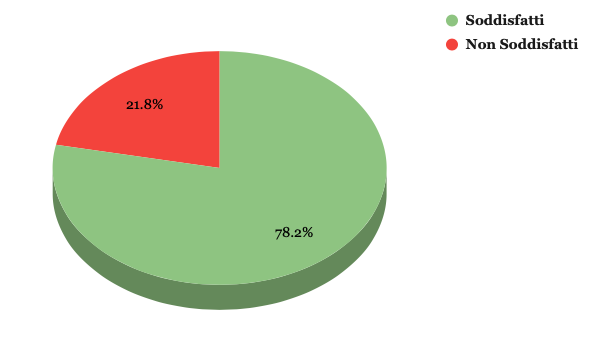
\includegraphics[width=0.7\textwidth]{img/RequisitiFunzionali.png}
    \caption{Grafico a torta che mostra la percentuale di soddisfacimento dei requisiti funzionali}
\end{figure}
\newpage
\subsection{Tracciamento requisiti di vincolo}

\begin{longtable}{|>{\centering\arraybackslash}m{0.08\textwidth}|>{\centering\arraybackslash}m{0.64\textwidth}|>{\centering\arraybackslash}m{0.18\textwidth}|}
	\hline
	\textbf{Codice} & \textbf{Descrizione} & \textbf{Stato}\\\hline
	\endfirsthead
	\hline
	\textbf{Codice} & \textbf{Descrizione} & \textbf{Stato}\\\hline
	\endhead
    \hline
    \textbf{RVO1} & Il chatbot deve rispondere con il contesto dato dai file di allenamento (pdf o file di testo inseriti) & Soddisfatto \\
    \hline
    \textbf{RVO2} & \href{https://code7crusaders.github.io/docs/PB/documentazione_interna/glossario.html#llm-large-language-model}{LLM\textsuperscript{G}} deve essere integrato tramite API & Soddisfatto \\
    \hline
    \textbf{RVO3} & \href{https://code7crusaders.github.io/docs/PB/documentazione_interna/glossario.html#llm-large-language-model}{LLM\textsuperscript{G}} utilizzato deve essere quello di OpenAI & Soddisfatto \\
    \hline
    \textbf{RVO4} & Deve essere usato un database relazionale & Soddisfatto \\
    \hline
    \textbf{RVO5} & Deve essere gestito il salvataggio delle chat precedenti con tutti i messaggi in esse tramite un database relazionale con \href{https://code7crusaders.github.io/docs/PB/documentazione_interna/glossario.html#postgresql}{PostgreSQL\textsuperscript{G}} & Soddisfatto \\
    \hline
    \textbf{RVO6} & Deve essere implementato un database vettoriale & Soddisfatto \\
    \hline
    \textbf{RVO7} & Deve essere implementato un database vettoriale \href{https://code7crusaders.github.io/docs/PB/documentazione_interna/glossario.html#faiss}{FAISS\textsuperscript{G}} per poter rendere possibile la ricerca con contesto dall'\href{https://code7crusaders.github.io/docs/PB/documentazione_interna/glossario.html#llm-large-language-model}{LLM\textsuperscript{G}} & Soddisfatto \\
    \hline
    \textbf{RVO8} & Deve essere implementato un embedding model & Soddisfatto \\
    \hline
    \textbf{RVO9} & L'embedding model deve essere quello di OpenAI & Soddisfatto \\
    \hline
    \textbf{RVO10} & Deve essere implementata una WebApp che permetta di comunicare con il chatbot & Soddisfatto \\
    \hline
    \textbf{RVO11} & L’interfaccia deve essere costruita utilizzando componenti funzionali React & Soddisfatto \\
    \hline
    \textbf{RVO12} & Si deve creare un backend che gestisca le chiamate HTTP, il database vettoriale e il database relazionale con Flask & Soddisfatto \\
    \hline
    \textbf{RVO13} & La gestione dello stato locale deve essere implementata tramite useState & Soddisfatto \\
    \hline
    \textbf{RVO14} & La WebApp deve utilizzare React Router per gestire la navigazione tra le pagine & Soddisfatto \\
    \hline
    \textbf{RVO15} & Gli stili devono essere gestiti tramite CSS inline o con className per garantire modularità & Soddisfatto \\
    \hline
    \textbf{RVO16} & La comunicazione tra componenti deve essere gestita inviando funzioni come props & Soddisfatto \\
    \hline
    \textbf{RVO17} & La WebApp deve essere responsiva e adattarsi dinamicamente alle dimensioni della finestra & Soddisfatto \\
    \hline
    \textbf{RVO18} & La gestione dei blocchi di testo vettorializzati deve essere gestita tramite Faiss & Soddisfatto \\
    \hline
    \textbf{RVD19} & Le metriche delle run del chatbot devono essere recuperate tramite Langsmith & Soddisfatto \\
    \hline
    \textbf{RVO20} & Bisogna usare la libreria \href{https://code7crusaders.github.io/docs/PB/documentazione_interna/glossario.html#langchain}{LangChain\textsuperscript{G}} per la interazione con i modelli \href{https://code7crusaders.github.io/docs/PB/documentazione_interna/glossario.html#llm-large-language-model}{LLM\textsuperscript{G}} e \href{https://code7crusaders.github.io/docs/PB/documentazione_interna/glossario.html#embedding}{Embedding\textsuperscript{G}} & Soddisfatto \\
    \hline
\caption{Tabella Requisiti di vincolo soddisfatti}
\end{longtable}

\begin{figure}[H]
    \centering
    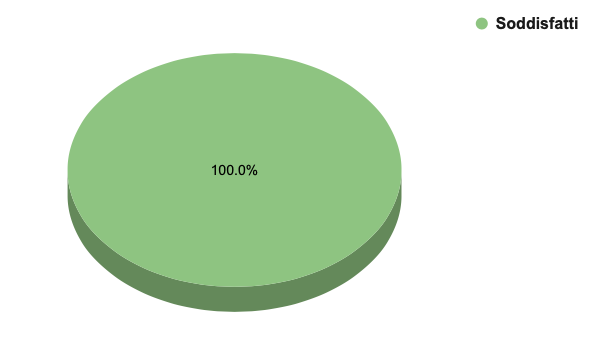
\includegraphics[width=0.7\textwidth]{img/RequisitiVincolo.png}
    \caption{Grafico a torta che mostra la percentuale di soddisfacimento dei requisiti di vincolo}
\end{figure}

\newpage
\subsection{Tracciamento requisiti di qualità}

\begin{longtable}{|>{\centering\arraybackslash}m{0.08\textwidth}|>{\centering\arraybackslash}m{0.64\textwidth}|>{\centering\arraybackslash}m{0.18\textwidth}|}
	\hline
	\textbf{Codice} & \textbf{Descrizione} & \textbf{Stato}\\\hline
	\endfirsthead
	\hline
	\textbf{Codice} & \textbf{Descrizione} & \textbf{Stato}\\\hline
	\endhead
	\hline
    \textbf{RQO1} & Schema di progettazione della base di dati & Soddisfatto \\
    \hline
    \textbf{RQO2} & Codice prodotto in formato sorgente reso disponibile tramite repository pubblici & Soddisfatto \\
    \hline
    \textbf{RQO3} & Documentazione riassuntiva delle metriche e dei risultati & Soddisfatto \\
    \hline
    \textbf{RQO4} & Il software deve essere testato con una copertura di codice minima dell'80\% e una copertura dei rami dell'80\%, con un obiettivo ottimale del 100\% & Soddisfatto \\
    \hline
    \textbf{RQO5} & Il 90\% dei test deve essere superato come requisito minimo, mentre l'obiettivo ottimale è il 100\% & Soddisfatto \\
    \hline
    \textbf{RQO6} & La metodologia di sviluppo deve seguire il paradigma del Test Driven Development (TDD), garantendo che il codice venga scritto partendo dai test & Soddisfatto \\
    \hline

\caption{Tabella Requisiti di qualità soddisfatti}
\end{longtable}

\begin{figure}[H]
    \centering
    \includegraphics[width=0.7\textwidth]{img/RequisitiQualità.png}
    \caption{Grafico a torta che mostra la percentuale di soddisfacimento dei requisiti di qualità}
\end{figure}
\newpage

\subsection{Soddisfazione totale dei requisiti}
Il gruppo Code7Crusaders ha soddisfatto 69 su 81, arrivando ad una copertura del \textbf{85.2\%}.
\begin{center}
\begin{tabular}{|c|c|}
\hline
\textbf{Soddisfatti} & \textbf{Non soddisfatti} \\
\hline
69 & 12 \\
\hline
\end{tabular}
\end{center}
\begin{figure}[H]
    \centering
    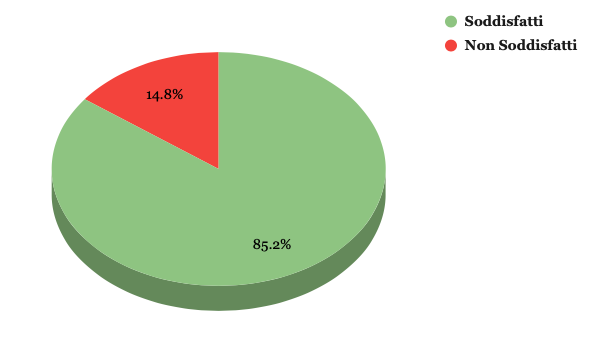
\includegraphics[width=0.7\textwidth]{img/RequisitiTotali.png}
    \caption{Grafico a torta dei Requisiti soddisfatti rispetto al totale}
\end{figure}
Per quanto riguarda la copertura dei requisiti obbligatori, la copertura rilevata è di 66 su 66 requisiti, arrivando quindi ad un \textbf{100\%} sul totale.
\begin{center}
\begin{tabular}{|c|c|}
\hline
\textbf{Soddisfatti} & \textbf{Non soddisfatti} \\
\hline
66 & 0 \\
\hline
\end{tabular}
\end{center}
\begin{figure}[H]
    \centering
    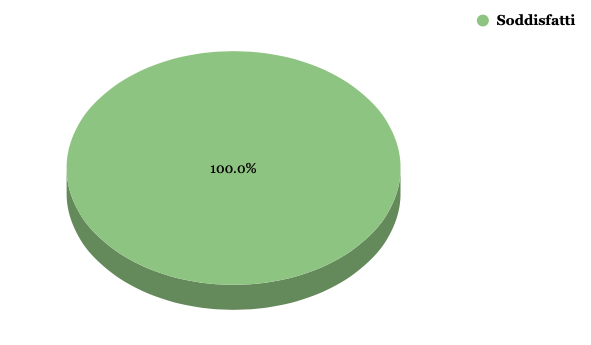
\includegraphics[width=0.7\textwidth]{img/RequisitiObbligatori.png}
    \caption{Grafico a torta dei Requisiti obbligatori soddisfatti rispetto al totale}
\end{figure}
\newpage
In termini di soddisfacimento dei requisiti desiderabili, è stata raggiunta una copertura del \textbf{66.67\%}, con 2 su 3.
\begin{center}
\begin{tabular}{|c|c|}
\hline
\textbf{Soddisfatti} & \textbf{Non soddisfatti} \\
\hline
2 & 1 \\
\hline
\end{tabular}
\end{center}

\begin{figure}[H]
    \centering
    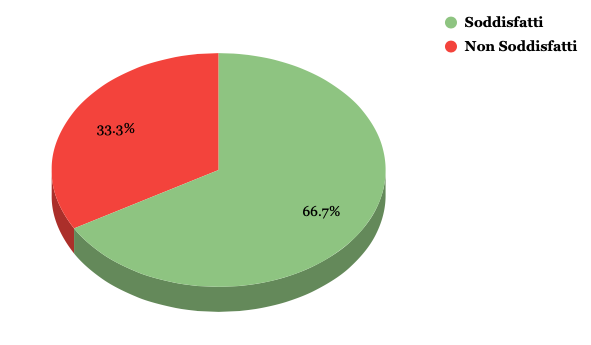
\includegraphics[width=0.7\textwidth]{img/RequisitiDesiderabili.png}
    \caption{Grafico a torta dei Requisiti desiderabili soddisfatti rispetto al totale}
\end{figure}

Per quanto concerne l’adempimento dei requisiti facoltativi, abbiamo conseguito una percentuale del \textbf{8.3\%} sul totale, con 1 su 12 requisiti considerati.
\begin{center}
    \begin{tabular}{|c|c|}
    \hline
    \textbf{Soddisfatti} & \textbf{Non soddisfatti} \\
    \hline
    1 & 11 \\
    \hline
    \end{tabular}
    \end{center}

    \begin{figure}[H]
        \centering
        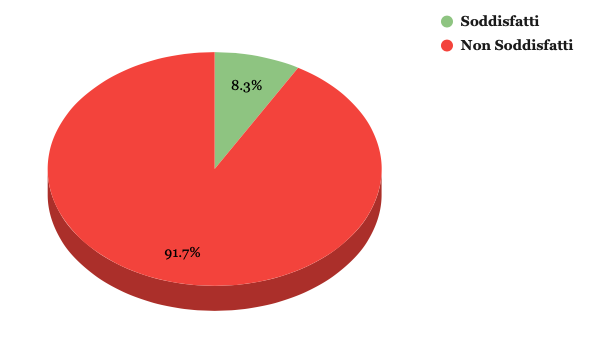
\includegraphics[width=0.7\textwidth]{img/RequisitiFacoltativi.png}
        \caption{Grafico a torta dei Requisiti facoltativi soddisfatti rispetto al totale}
    \end{figure}
